\documentclass[../Main.tex]{subfiles}

\graphicspath{{\subfix{../Figures_and_Tables/}}}
 
\begin{document}

\newpage
\begin{figure}[t]
	\begin{center}
	\caption{\label{fig:q_nursing_homes_trends} \centering Trends in the Quantity of Nursing Homes Per 100,000}
    \begin{subfigure}[b]{\textwidth} \centering
    \caption{Pennsylvania}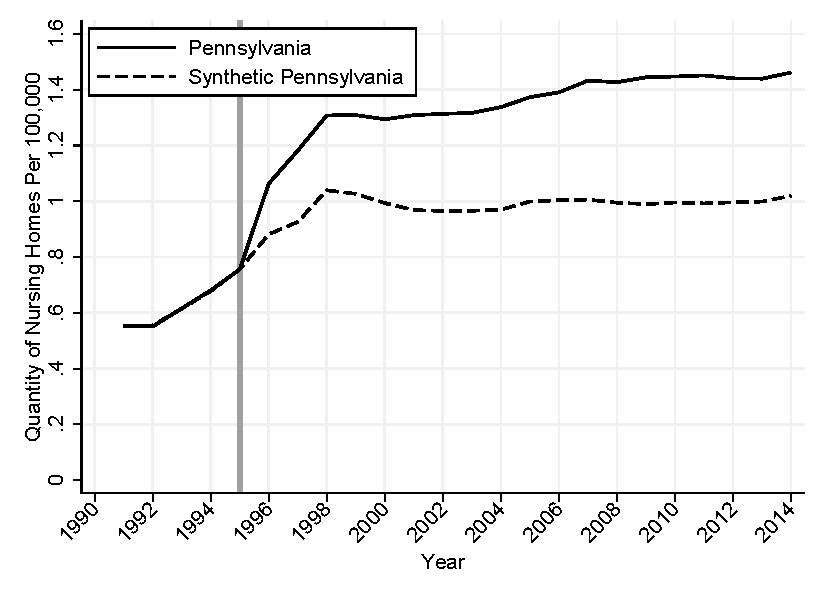
\includegraphics[width=.48\textwidth,keepaspectratio]{q_nursing_homes_Trends_PA.pdf}
    \end{subfigure}\\
    \vspace{.4cm}
    \begin{subfigure}[b]{.48\textwidth} \centering
    \caption{Indiana}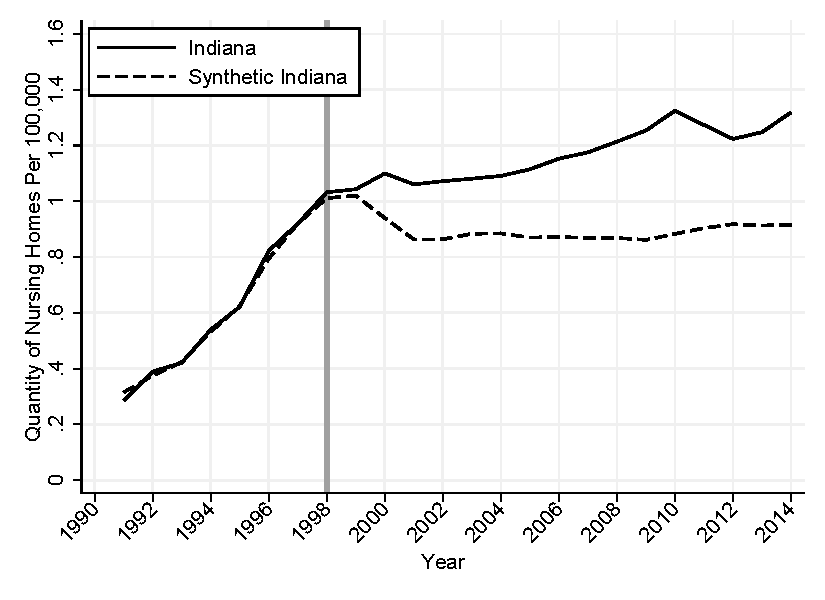
\includegraphics[width=\textwidth,keepaspectratio]{q_nursing_homes_Trends_IN.pdf}
    \end{subfigure}\quad%
    \begin{subfigure}[b]{.48\textwidth} \centering
    \caption{North Dakota}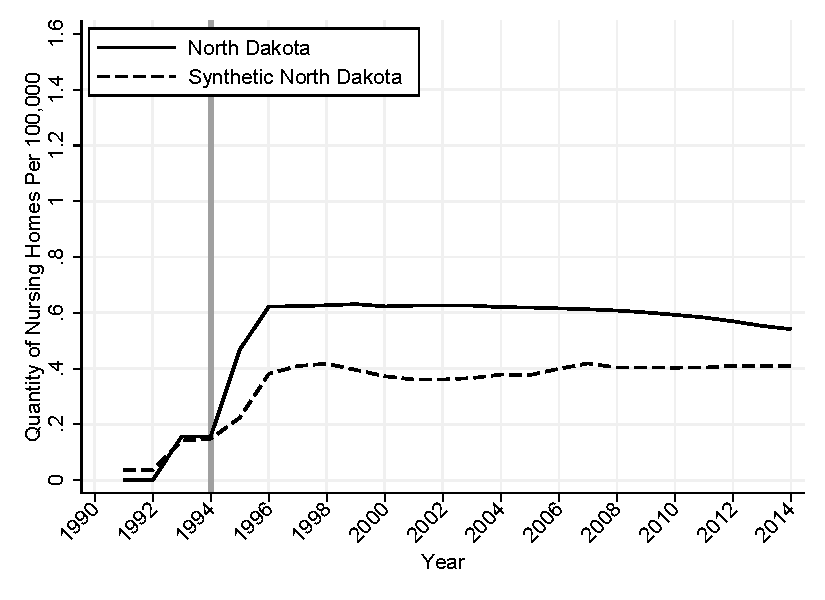
\includegraphics[width=\textwidth,keepaspectratio]{q_nursing_homes_Trends_ND.pdf}
    \end{subfigure}
    \end{center}
    \footnotesize
		\textit{Notes}: This figure shows trends over time in the quantity of nursing homes per 100,000 in PA, IN, and ND and their respective synthetic controls. The vertical lines represent the year in which each state dropped NH-CON regulations. Data source: 1991-2014 Centers for Medicare and Medicaid Services’ (CMS) Provider of Services files.
\end{figure}
\clearpage


\newpage
\begin{figure}[t]
	\begin{center}
	\caption{\label{fig:q_nursing_homes_gaps} \centering Year-Specific Effects of Dropping NH-CON on the Quantity of Nursing Homes Per 100,000 ($\hat{\alpha}_{1t}$)}
    \begin{subfigure}[b]{\textwidth} \centering
    \caption{Pennsylvania}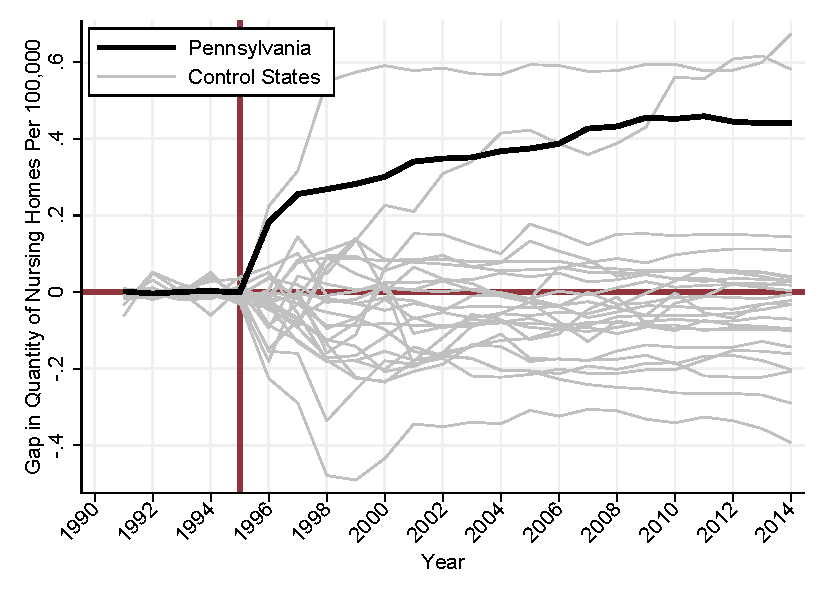
\includegraphics[width=.48\textwidth,keepaspectratio]{q_nursing_homes_Gaps_with_Placebos_20_PA.pdf}
    \end{subfigure}\\
    \vspace{.4cm}
    \begin{subfigure}[b]{.48\textwidth} \centering
    \caption{Indiana}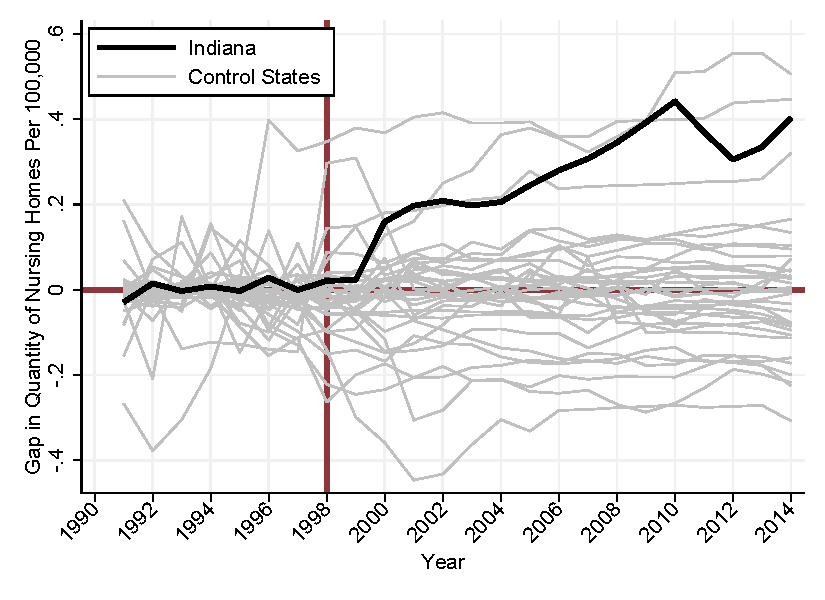
\includegraphics[width=\textwidth,keepaspectratio]{q_nursing_homes_Gaps_with_Placebos_20_IN.pdf}
    \end{subfigure}\quad%
    \begin{subfigure}[b]{.48\textwidth} \centering
    \caption{North Dakota}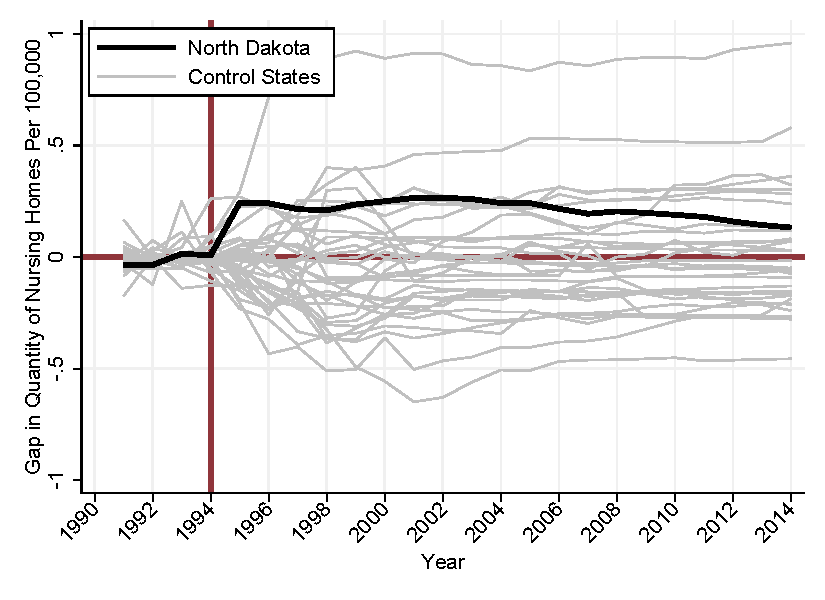
\includegraphics[width=\textwidth,keepaspectratio]{q_nursing_homes_Gaps_with_Placebos_20_ND.pdf}
    \end{subfigure}
    \end{center}
    \footnotesize
		\textit{Notes}: The solid black lines in this figure represent the year-specific effects of dropping NH-CON regulations on the quantity of nursing homes per 100,000 in PA, IN, and ND ($\hat{\alpha}_{1t}$ from equation (\ref{eq:year_spec_effect})). The light gray lines represent the year-specific placebo effects for the states in the donor pool of potential control states. We only show states that have a relatively good fit in the pre-treatment period by dropping states from the figure with an $RMSPE_i^{pre}$ more than twenty times the $RMSPE_i^{pre}$ of the treated states \citep{abadie2010synthetic}. The vertical lines represent the year in which each state dropped NH-CON regulations. Data source: 1980-2014 National Health Expenditure Accounts (NHEA).
\end{figure}
\clearpage


\newpage
\begin{figure}[t]
	\begin{center}
	\caption{\label{fig:q_nursing_home_beds_trends} \centering Trends in the Quantity of Nursing Home Beds Per 100,000}
    \begin{subfigure}[b]{\textwidth} \centering
    \caption{Pennsylvania}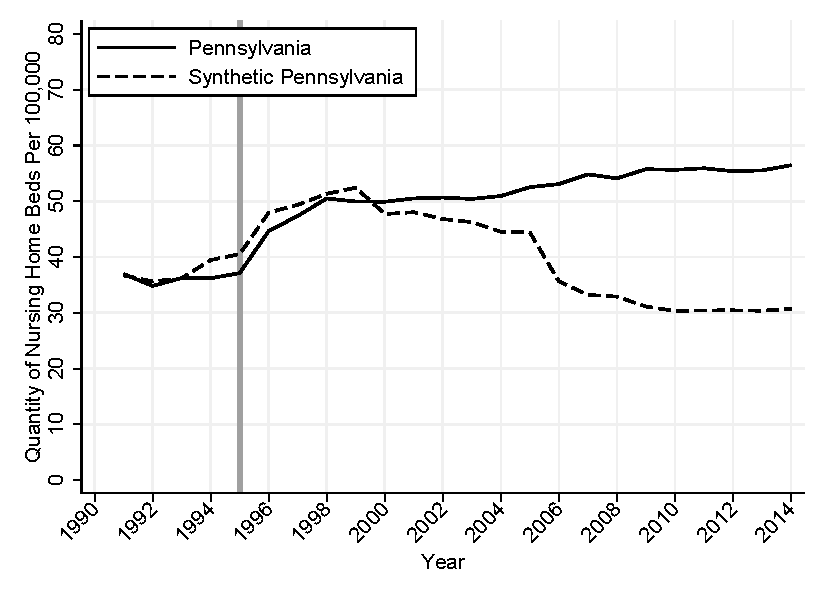
\includegraphics[width=.48\textwidth,keepaspectratio]{q_nursing_home_beds_Trends_PA.pdf}
    \end{subfigure}\\
    \vspace{.4cm}
    \begin{subfigure}[b]{.48\textwidth} \centering
    \caption{Indiana}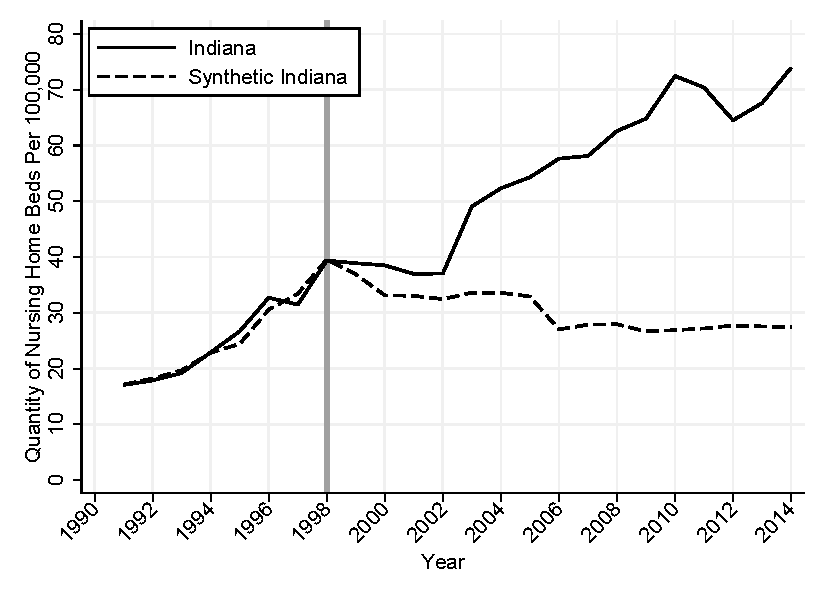
\includegraphics[width=\textwidth,keepaspectratio]{q_nursing_home_beds_Trends_IN.pdf}
    \end{subfigure}\quad%
    \begin{subfigure}[b]{.48\textwidth} \centering
    \caption{North Dakota}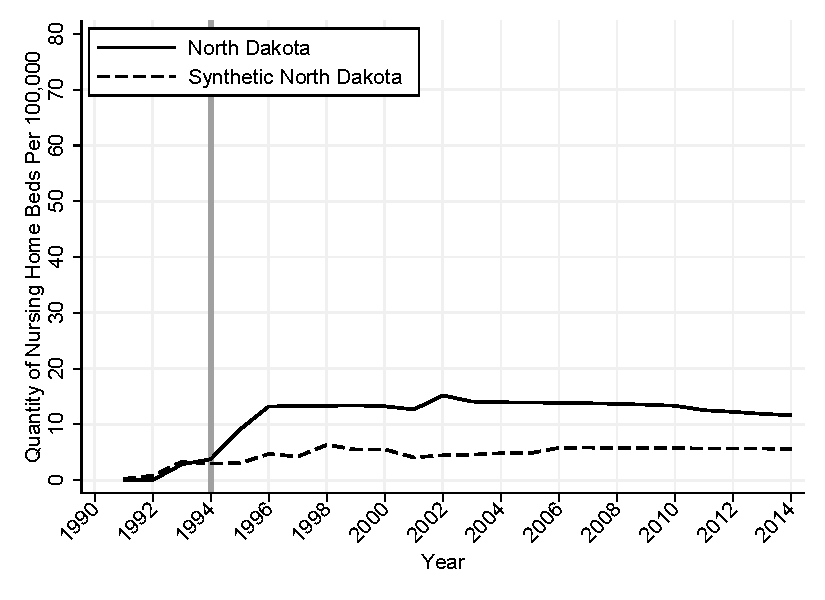
\includegraphics[width=\textwidth,keepaspectratio]{q_nursing_home_beds_Trends_ND.pdf}
    \end{subfigure}
    \end{center}
    \footnotesize
		\textit{Notes}: This figure shows trends over time in the quantity of nursing home beds per 100,000 in PA, IN, and ND and their respective synthetic controls. The vertical lines represent the year in which each state dropped NH-CON regulations. Data source: 1991-2014 Centers for Medicare and Medicaid Services’ (CMS) Provider of Services files.
\end{figure}
\clearpage


\newpage
\begin{figure}[t]
	\begin{center}
	\caption{\label{fig:q_nursing_home_beds_gaps} \centering Year-Specific Effects of Dropping NH-CON on the Quantity of Nursing Home Beds Per 100,000 ($\hat{\alpha}_{1t}$)}
    \begin{subfigure}[b]{\textwidth} \centering
    \caption{Pennsylvania}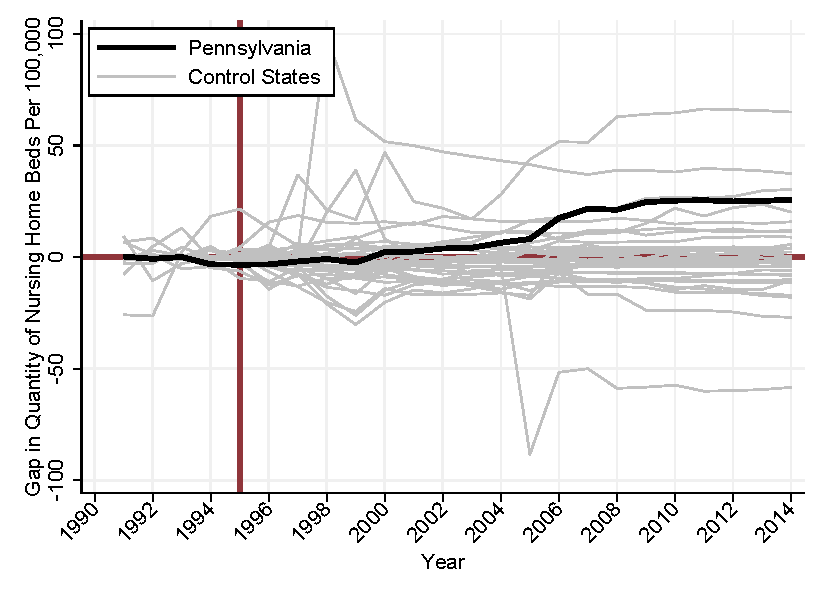
\includegraphics[width=.48\textwidth,keepaspectratio]{q_nursing_home_beds_Gaps_with_Placebos_20_PA.pdf}
    \end{subfigure}\\
    \vspace{.4cm}
    \begin{subfigure}[b]{.48\textwidth} \centering
    \caption{Indiana}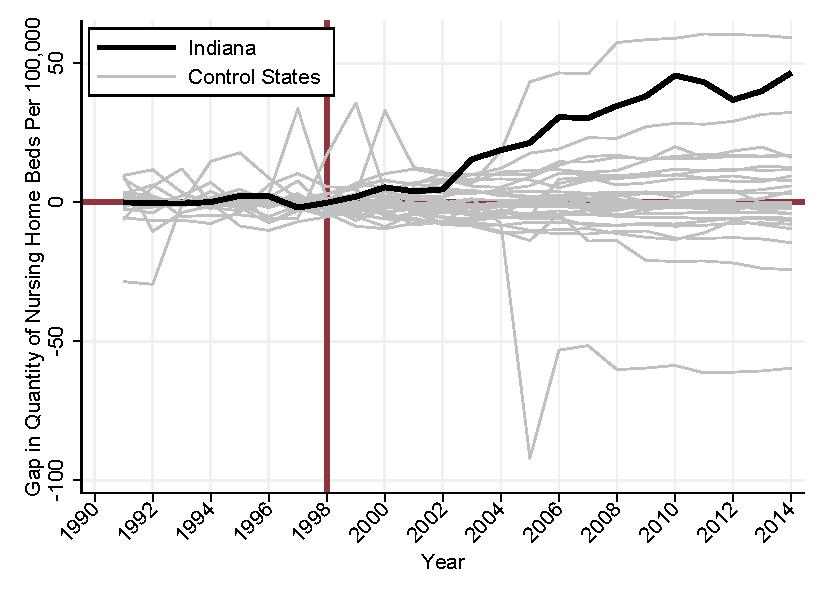
\includegraphics[width=\textwidth,keepaspectratio]{q_nursing_home_beds_Gaps_with_Placebos_20_IN.pdf}
    \end{subfigure}\quad%
    \begin{subfigure}[b]{.48\textwidth} \centering
    \caption{North Dakota}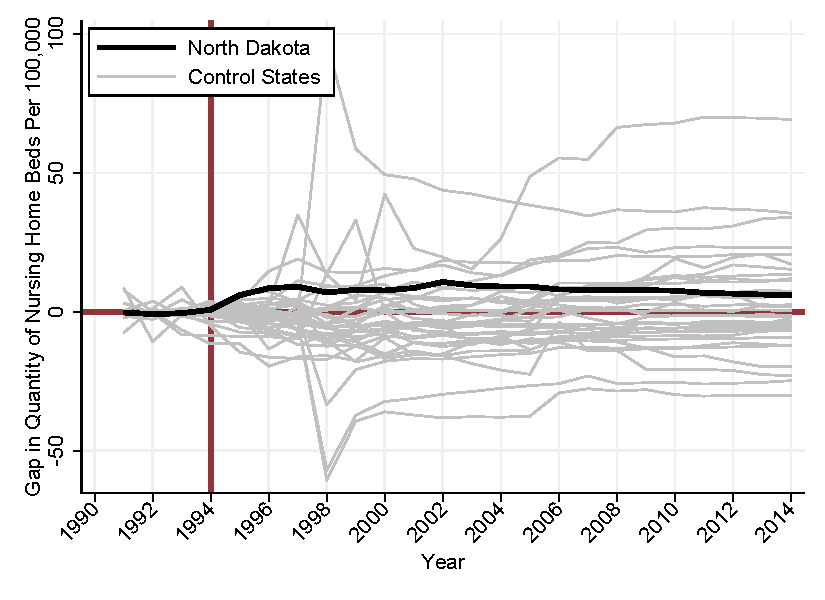
\includegraphics[width=\textwidth,keepaspectratio]{q_nursing_home_beds_Gaps_with_Placebos_20_ND.pdf}
    \end{subfigure}
    \end{center}
    \footnotesize
		\textit{Notes}: The solid black lines in this figure represent the year-specific effects of dropping NH-CON regulations on the quantity of nursing home beds per 100,000 in PA, IN, and ND ($\hat{\alpha}_{1t}$ from equation (\ref{eq:year_spec_effect})). The light gray lines represent the year-specific placebo effects for the states in the donor pool of potential control states. We only show states that have a relatively good fit in the pre-treatment period by dropping states from the figure with an $RMSPE_i^{pre}$ more than twenty times the $RMSPE_i^{pre}$ of the treated states \citep{abadie2010synthetic}. The vertical lines represent the year in which each state dropped NH-CON regulations. Data source: 1980-2014 National Health Expenditure Accounts (NHEA).
\end{figure}
\clearpage

\newpage
\begin{figure}[t]
	\begin{center}
	\caption{\label{fig:tot_exp_trends} \centering Trends in Total Nursing Home Expenditure Per Capita}
    \begin{subfigure}[b]{\textwidth} \centering
    \caption{Pennsylvania}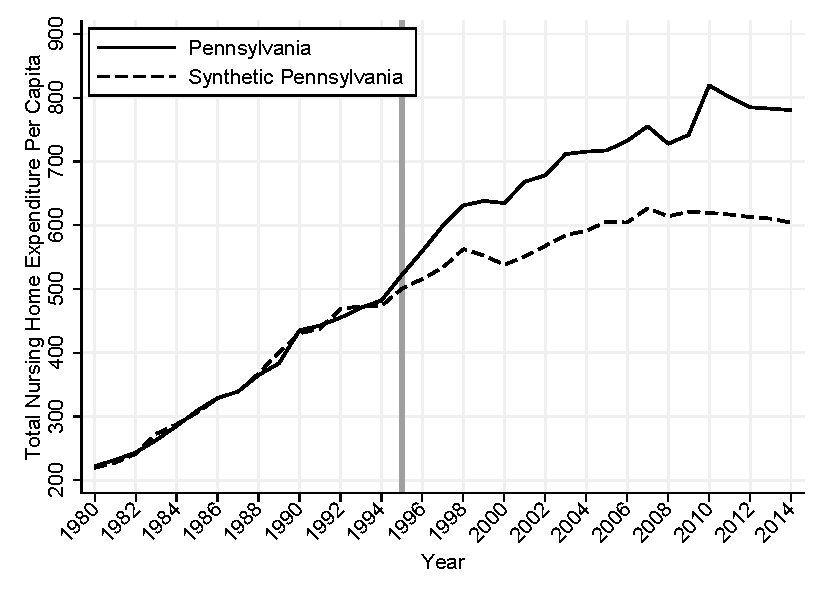
\includegraphics[width=.48\textwidth,keepaspectratio]{nursing_home_tot_exp_Trends_PA.pdf}
    \end{subfigure}\\
    \vspace{.4cm}
    \begin{subfigure}[b]{.48\textwidth} \centering
    \caption{Indiana}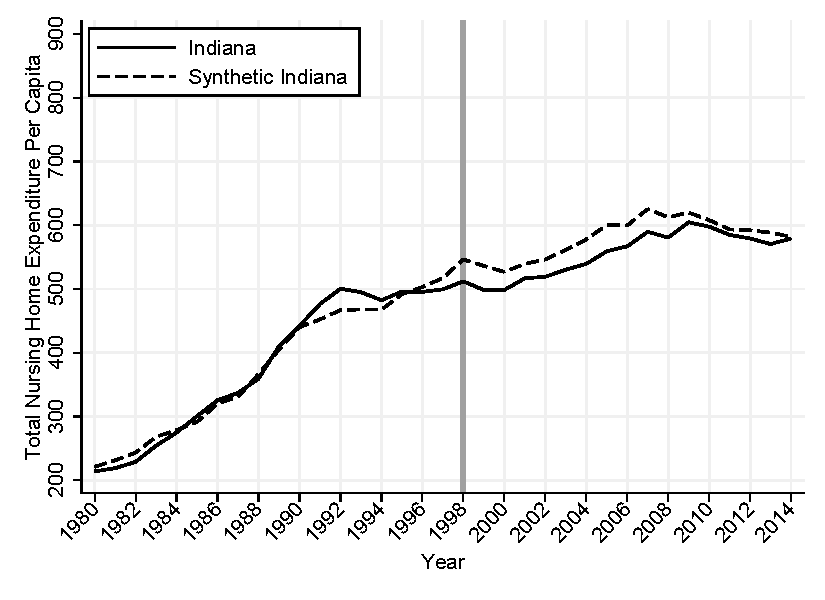
\includegraphics[width=\textwidth,keepaspectratio]{nursing_home_tot_exp_Trends_IN.pdf}
    \end{subfigure}\quad%
    \begin{subfigure}[b]{.48\textwidth} \centering
    \caption{North Dakota}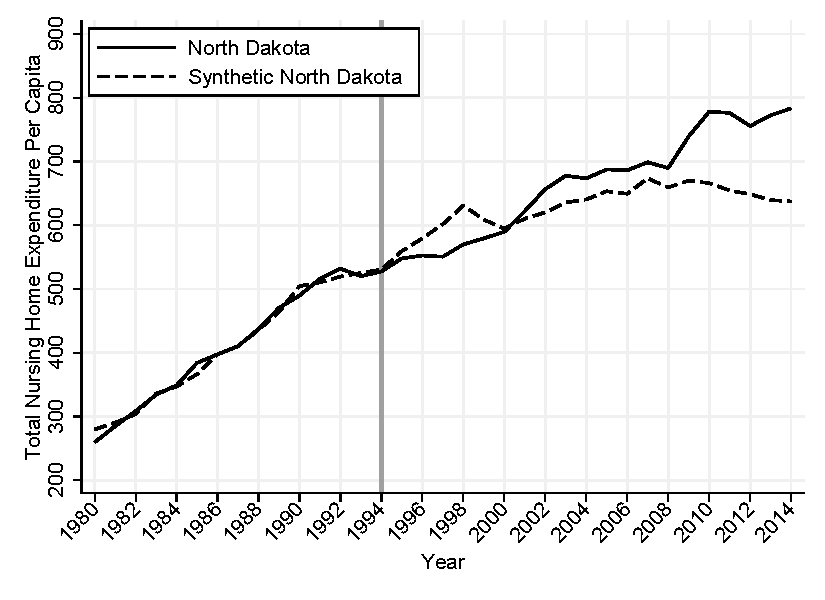
\includegraphics[width=\textwidth,keepaspectratio]{nursing_home_tot_exp_Trends_ND.pdf}
    \end{subfigure}
    \end{center}
    \footnotesize
		\textit{Notes}: This figure shows trends over time in total nursing home expenditure per capita in PA, IN, and ND and their respective synthetic controls. The vertical lines represent the year in which each state dropped NH-CON regulations. Data source: 1980-2014 National Health Expenditure Accounts (NHEA).
\end{figure}
\clearpage



\newpage
\begin{figure}[t]
	\begin{center}
	\caption{\label{fig:tot_exp_gaps} \centering Year-Specific Effects of Dropping NH-CON on Total Expenditure Per Capita ($\hat{\alpha}_{1t}$)}
    \begin{subfigure}[b]{\textwidth} \centering
    \caption{Pennsylvania}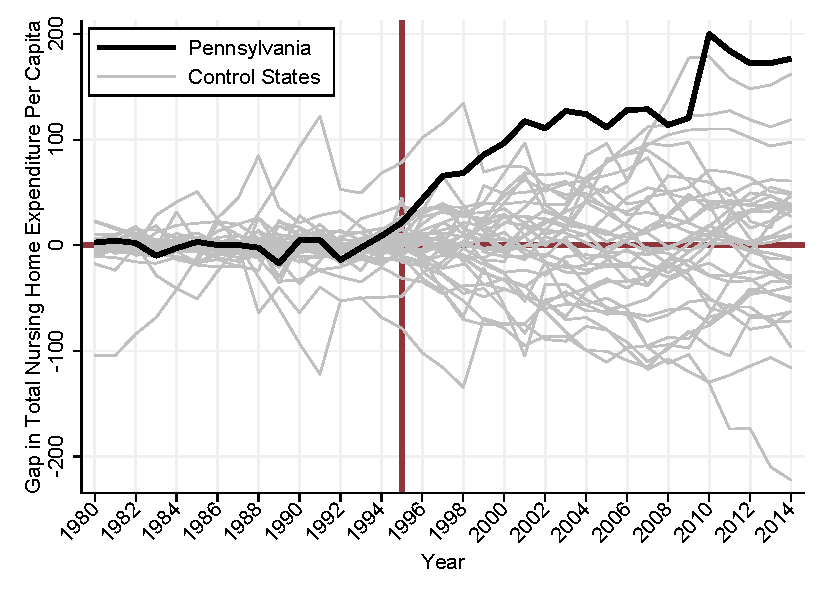
\includegraphics[width=.48\textwidth,keepaspectratio]{nursing_home_tot_exp_Gaps_with_Placebos_20_PA.pdf}
    \end{subfigure}\\
    \vspace{.4cm}
    \begin{subfigure}[b]{.48\textwidth} \centering
    \caption{Indiana}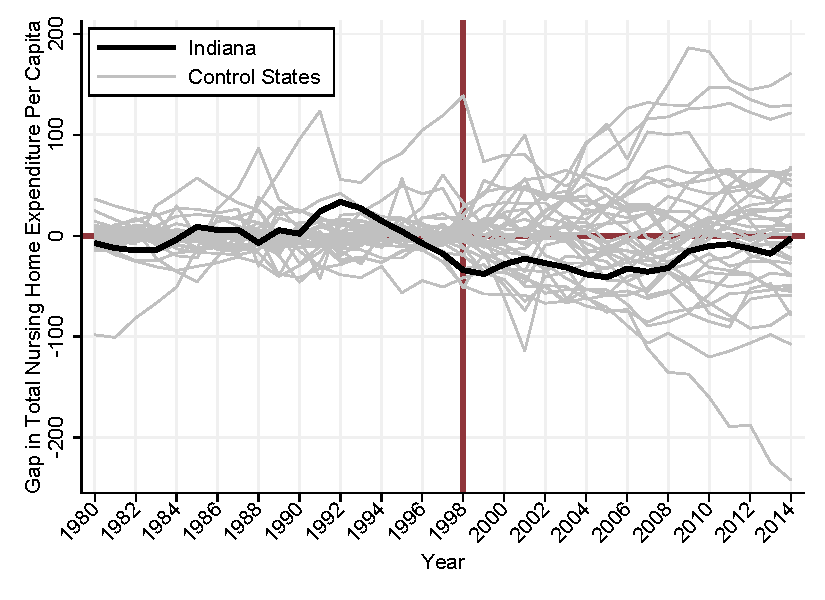
\includegraphics[width=\textwidth,keepaspectratio]{nursing_home_tot_exp_Gaps_with_Placebos_20_IN.pdf}
    \end{subfigure}\quad%
    \begin{subfigure}[b]{.48\textwidth} \centering
    \caption{North Dakota}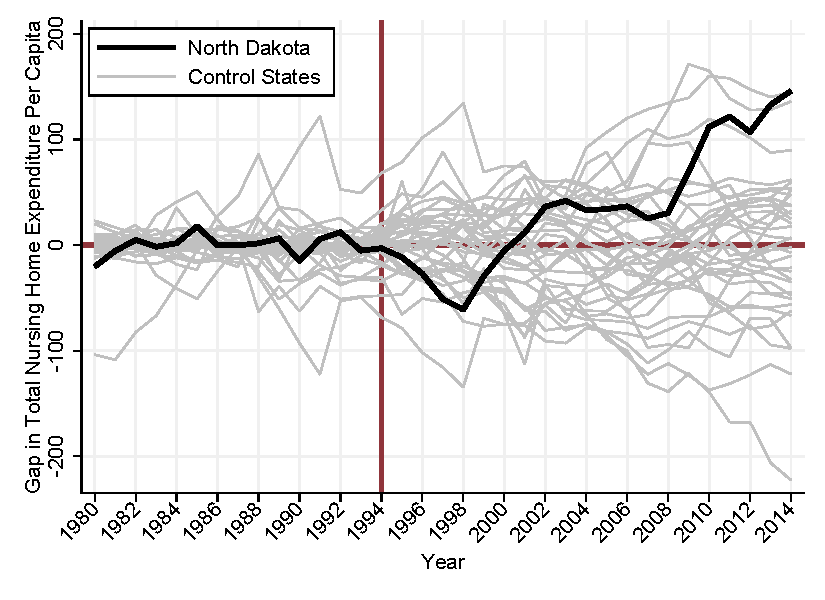
\includegraphics[width=\textwidth,keepaspectratio]{nursing_home_tot_exp_Gaps_with_Placebos_20_ND.pdf}
    \end{subfigure}
    \end{center}
    \footnotesize
		\textit{Notes}: The solid black lines in this figure represent the year-specific effects of dropping NH-CON regulations on total nursing home expenditure per capita in PA, IN, and ND ($\hat{\alpha}_{1t}$ from equation (\ref{eq:year_spec_effect})). The light gray lines represent the year-specific placebo effects for the states in the donor pool of potential control states. We only show states that have a relatively good fit in the pre-treatment period by dropping states from the figure with an $RMSPE_i^{pre}$ more than twenty times the $RMSPE_i^{pre}$ of the treated states \citep{abadie2010synthetic}. The vertical lines represent the year in which each state dropped NH-CON regulations. Data source: 1980-2014 National Health Expenditure Accounts (NHEA).
\end{figure}
\clearpage



\newpage
\begin{figure}[t]
	\begin{center}
	\caption{\label{fig:medicaid_exp_trends} \centering Trends in Nursing Home Medicaid Expenditure Per Capita}
    \begin{subfigure}[b]{\textwidth} \centering
    \caption{Pennsylvania}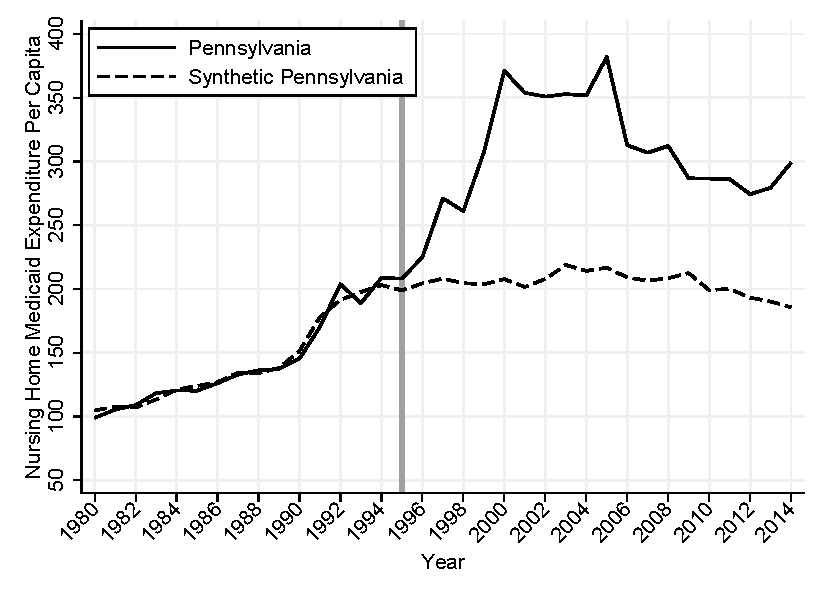
\includegraphics[width=.48\textwidth,keepaspectratio]{nursing_home_medicaid_exp_Trends_PA.pdf}
    \end{subfigure}\\
    \vspace{.4cm}
    \begin{subfigure}[b]{.48\textwidth} \centering
    \caption{Indiana}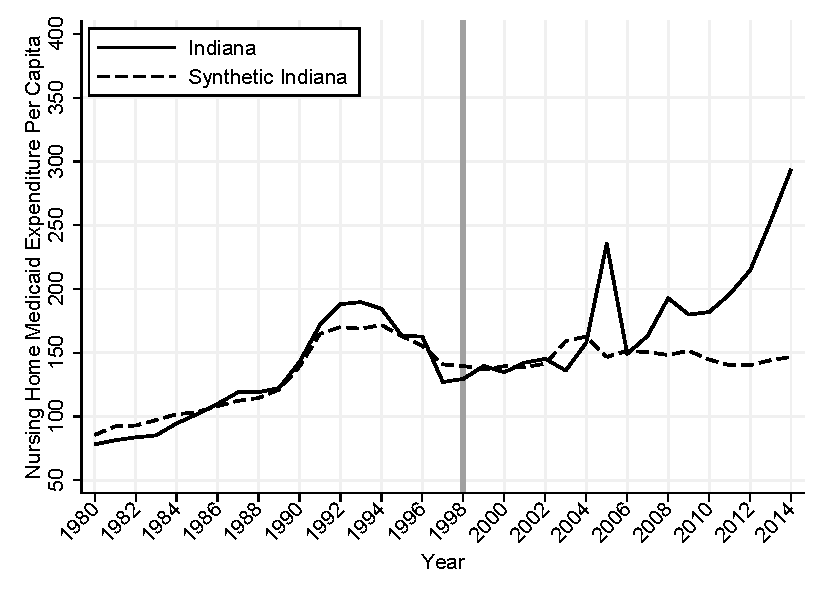
\includegraphics[width=\textwidth,keepaspectratio]{nursing_home_medicaid_exp_Trends_IN.pdf}
    \end{subfigure}\quad%
    \begin{subfigure}[b]{.48\textwidth} \centering
    \caption{North Dakota}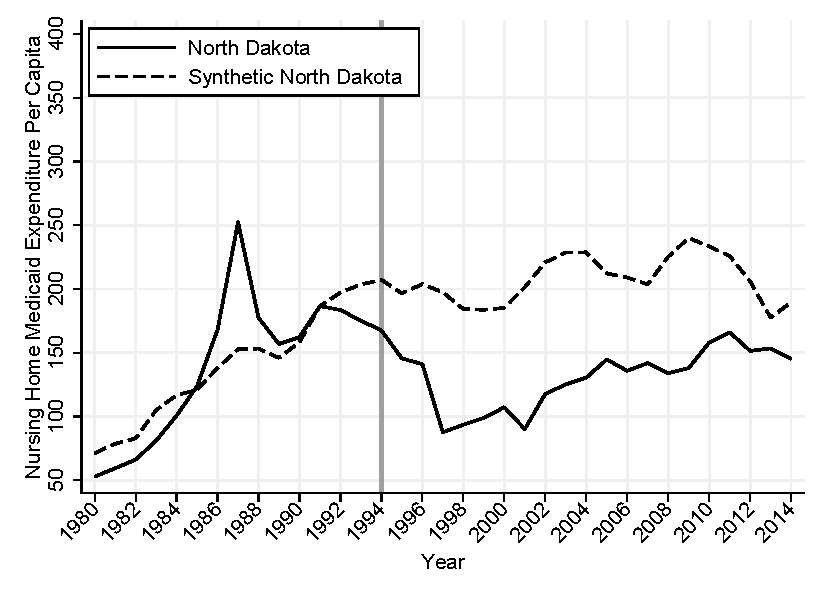
\includegraphics[width=\textwidth,keepaspectratio]{nursing_home_medicaid_exp_Trends_ND.pdf}
    \end{subfigure}
    \end{center}
    \footnotesize
		\textit{Notes}: This figure shows trends over time in nursing home medicaid expenditure per capita in PA, IN, and ND and their respective synthetic controls. The vertical lines represent the year in which each state dropped NH-CON regulations. Data source: 1980-2014 National Health Expenditure Accounts (NHEA).
\end{figure}
\clearpage



\newpage
\begin{figure}[t]
	\begin{center}
	\caption{\label{fig:medicaid_exp_gaps} \centering Year-Specific Effects of Dropping NH-CON on Medicaid Expenditure Per Capita ($\hat{\alpha}_{1t}$)}
    \begin{subfigure}[b]{\textwidth} \centering
    \caption{Pennsylvania}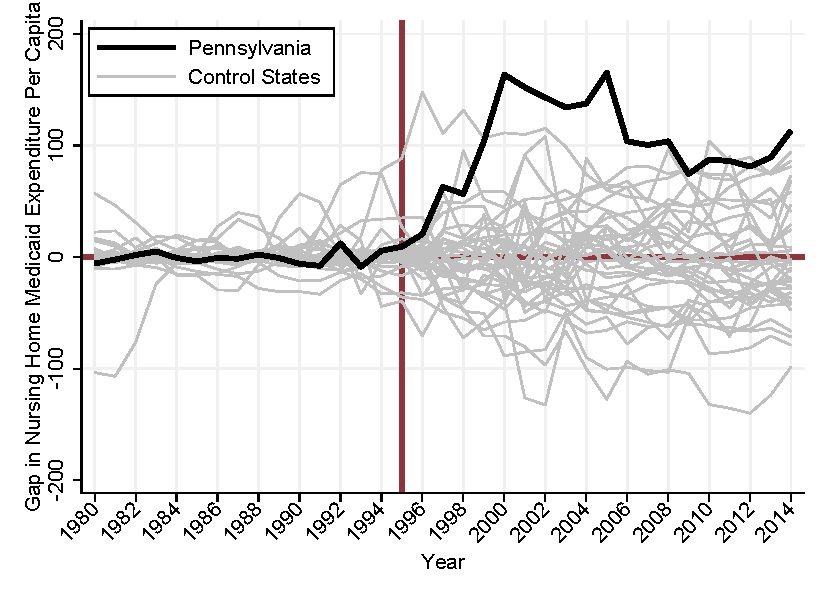
\includegraphics[width=.48\textwidth,keepaspectratio]{nursing_home_medicaid_exp_Gaps_with_Placebos_20_PA.pdf}
    \end{subfigure}\\
    \vspace{.4cm}
    \begin{subfigure}[b]{.48\textwidth} \centering
    \caption{Indiana}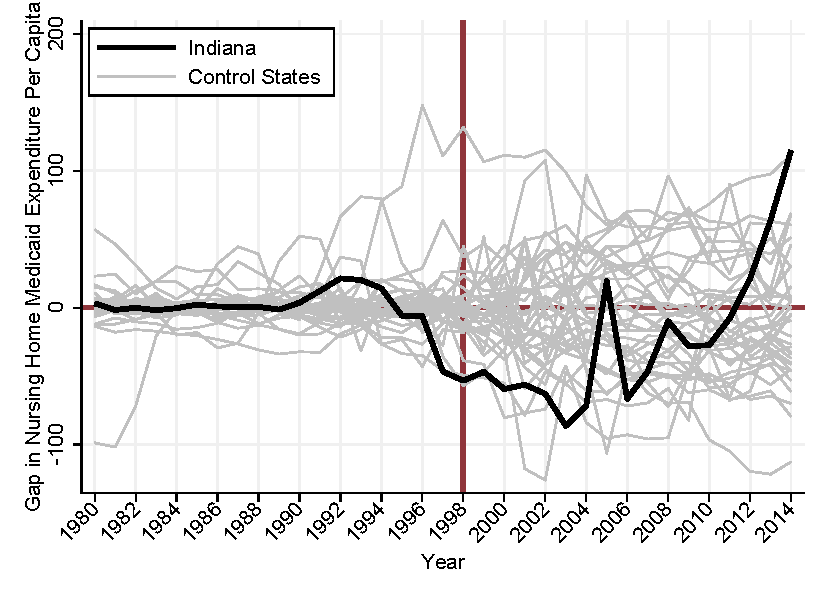
\includegraphics[width=\textwidth,keepaspectratio]{nursing_home_medicaid_exp_Gaps_with_Placebos_20_IN.pdf}
    \end{subfigure}\quad%
    \begin{subfigure}[b]{.48\textwidth} \centering
    \caption{North Dakota}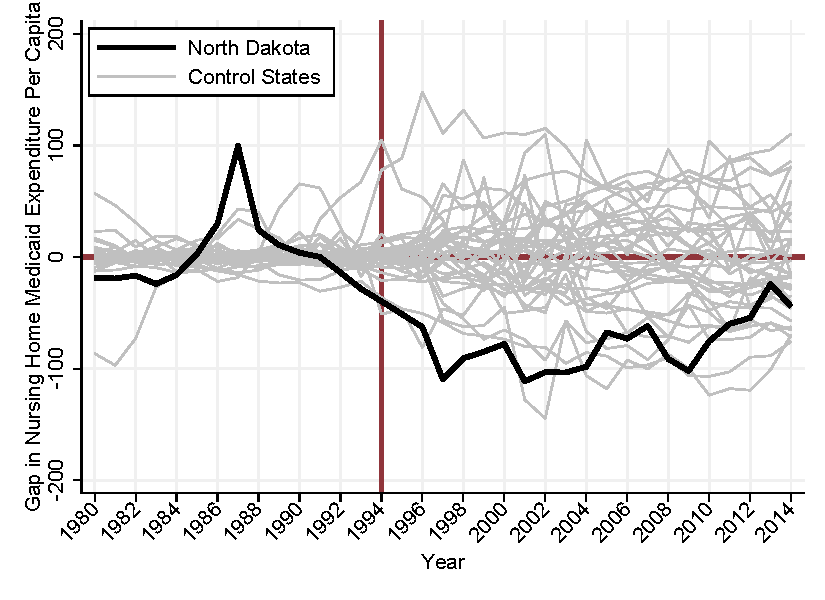
\includegraphics[width=\textwidth,keepaspectratio]{nursing_home_medicaid_exp_Gaps_with_Placebos_20_ND.pdf}
    \end{subfigure}
    \end{center}
    \footnotesize
		\textit{Notes}: The solid black lines in this figure represent the year-specific effects of dropping NH-CON regulations on nursing home medicaid expenditure per capita in PA, IN, and ND ($\hat{\alpha}_{1t}$ from equation (\ref{eq:year_spec_effect})). The light gray lines represent the year-specific placebo effects for the states in the donor pool of potential control states. We only show states that have a relatively good fit in the pre-treatment period by dropping states from the figure with an $RMSPE_i^{pre}$ more than twenty times the $RMSPE_i^{pre}$ of the treated states \citep{abadie2010synthetic}. The vertical lines represent the year in which each state dropped NH-CON regulations. Data source: 1980-2014 National Health Expenditure Accounts (NHEA).
\end{figure}
\clearpage

	


\end{document}